%% ==============================
\chapter{Implementation}
\label{sec:implementation}
%% ==============================
Questions to ask:
\begin{enumerate}
    \item Which frameworks from others do you use? (open source tools)
    \item Which algorithms do you use?
    \item Which programming language do you use and why did you choose it?
    \item What code patterns did you apply?
    \item How does the most relevant part of your code work? (Pseudocode?)
    \item Which parameters can be used for configuration?
    \item How did you find the used set of parameters?   
    \item What are the interfaces for the end user?
    \item How to use your work?
\end{enumerate}

What is the software or hardware system used to implement the research ideas? 

Which frameworks or approaches from previous work are used? 

What are the main design choices and trade-offs in your system? 

What are the main implementation challenges and solutions? 

(If relevant) Which algorithms are used? (With pseudocode) 

\begin{enumerate}
    \item Algorithms LIR, OpenCV, Watershed
    \item Structure of semantic hierarchical graphs
    \item ROS2 Nav stack
    \item Implementation on the real PeTRA Robot
    \item Operating a real elevator 
\end{enumerate}

The planner is implemented as a plugin for the \gls{ros_2} and is evaluated using realistic simulation scenarios and real-world experiments. The planner is designed to be modular and can be easily integrated with the existing navigation stack. The planner is also designed to be scalable and can be used in environments of varying sizes and complexity.

Python is used and libraries numpy, opencv, shaply

%% ==============================
\section{Hierarchy Creation}
\label{sec:hierarchy_creation}
%% ==============================

The input for hierarchy creation is the raw occupancy gridmap from the SLAMing process of the robot. For the evaluation and better comparison the same benchmark map as used for the algorithm from \cite{ryu_hierarchical_2020} is taken. For better readability the image of this raw occupancy gridmap from Chapter \ref{sec:benchmarks} is shown again here in Figure \ref{fig:freiburg_benchmark_2}.

\begin{figure}[h]
    \centering
    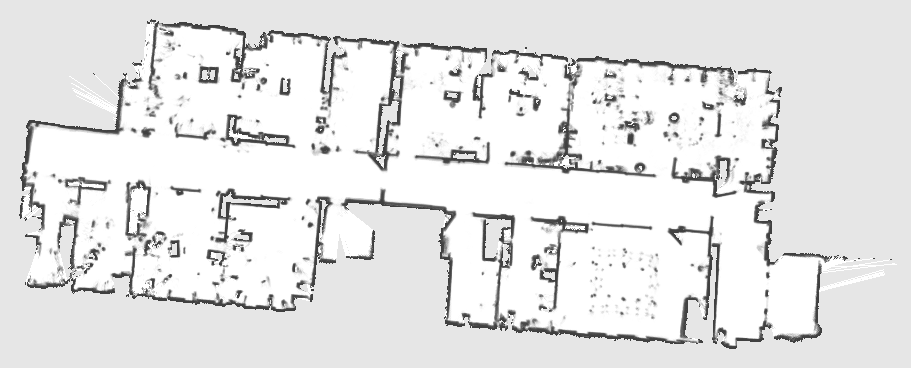
\includegraphics[width=0.75\textwidth]{figures/30_methods/freiburg_benchmark.png}
    \caption[The benchmark environment for hierarchy creation and straight path planning (intentional repetition)]{The benchmark environment for hierarchy creation and straight path planning recorded in the University of Freiburg (Source: \cite{cyrill_stachniss_robotics_2015})(intentional repetition)}
    \label{fig:freiburg_benchmark_2}
\end{figure}

This gridmap is build with the laser scanners of the mobile robot starting from the current pose at the time of starting the mapping. This starting pose is often not aligned with surrounding walls resulting in an apparent angle between the walls and the coordinate frame of the gridmap. This is not a problem for localization or path planning but makes it difficult to plan straight paths parallel to the walls. To solve this problem a rotation detection and outlier reduction algorithm is used.

\begin{figure}[h]
    \centering
    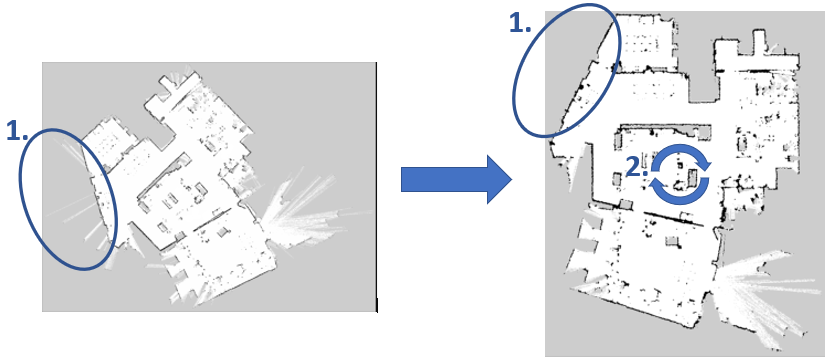
\includegraphics[width=0.75\textwidth]{figures/50_implementation/model_preprocessing_goal.png}
    \caption[Map preprocessing with rotation and outlier detection]{Map preprocessing with rotation and outlier detection. Original map on the left with outliers caused by transparent windows (1.). Resulting map on the right, outliers removed (1.) and rotation aligned with wall directions (2.) (Source: Tim Albert)}
    \label{fig:map_preprocessing}
\end{figure}

In Figure \ref{fig:map_preprocessing} the result of the preprocessing algorithm is seen. The algorithm first performs dilation and detects connected components. Based on the size these components are classified as outliers and the corresponding walls and white trails (see Figure \ref{fig:map_preprocessing} 1.) are removed. Then with the Probabilistic Hough Transform \cite{matas_robust_2000} straight lines are detected which represent the walls of the rooms. Finally the main orientation based on the most wall lines going in the same direction is chosen. To account for walls of one room and the adjacent wall perpendicular to it, the detected lines are clustered with the \gls{dbscan} algorithm \cite{ester_density-based_1996}. After obtaining the major rotation angle of the walls, the whole map is rotated to align with the coordinate frame of the gridmap. As this was developed and tested in an independent project it is not in the scope of this work.

The resulting map is now rotated parallel to the walls and outliers are removed. However there are still some artifacts in the map which obscure the real shape of the room. For best results some manual cleaning is still necessary. Most of these objects are dynamic obstacles which were at these positions during the mapping process but could be moved somewhere else by now. To not depend on this current snapshot of the environment the real shape of the room is estimated. The obstacles are later considered during the actual driving process. The task of the controller is to avoid these obstacles and provide a path around it. If this is not possible within the limits of the controller a replan is triggered. The resulting cleaned map is then binarized with a threshold and can bee seen in Figure \ref{fig:map_cleaned}

\begin{figure}[h]
    \centering
    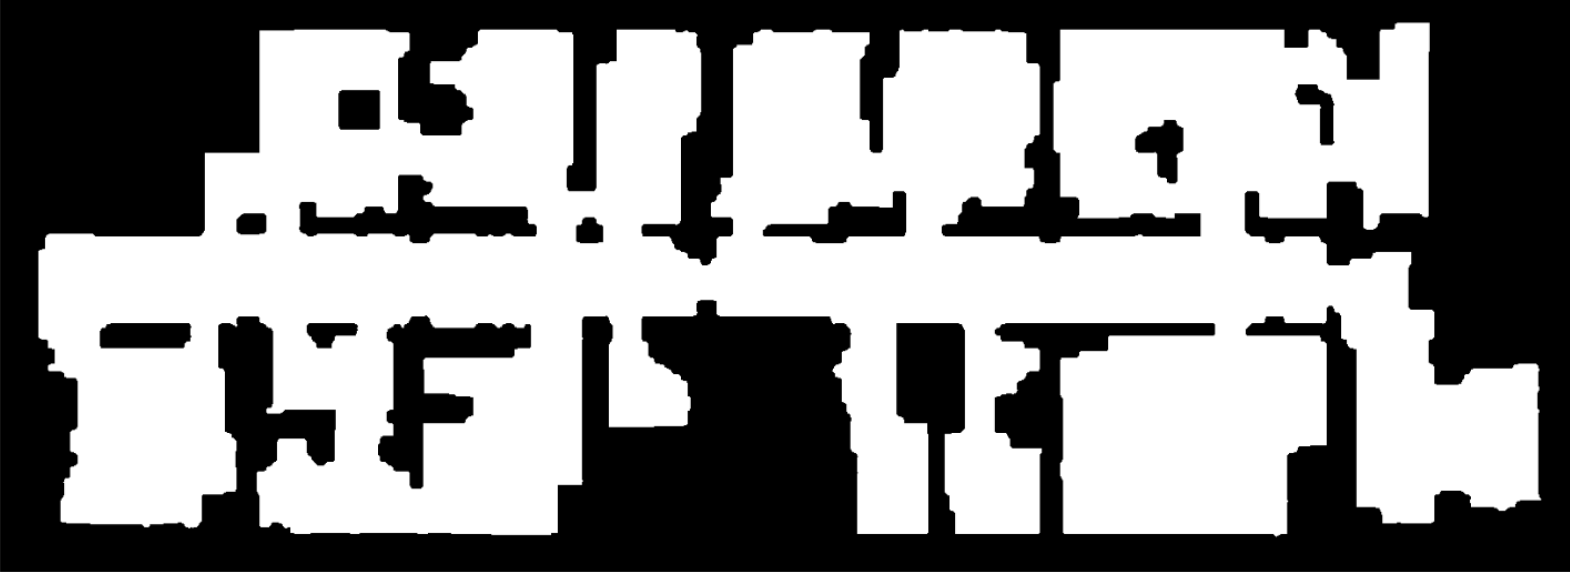
\includegraphics[width=0.75\textwidth]{figures/50_implementation/ryu.png}
    \caption[Binary map after rotation and manual cleaning]{Binary map after rotation and manual cleaning}
    \label{fig:map_cleaned}
\end{figure}

The segmentation of this map into single rooms and corridors is now done with the marker-controlled watershed algorithm \cite{parvati_image_2009}. For this the gridmap is converted into an numpy matrix and processed with opencv. OpenCV offers implementations for common image processing operations in python with which the watershed representation can be created. The process starts creating markers with which the normal watershed algorithm can be improved. Without predefined markers, watershed results in an over segmentation. For this an distance transform is performed on the image from Figure \ref{fig:map_cleaned}. This creates a mapping of each white pixels distance to the nearest black pixel. This can be interpreted as the obstacle clearance of this position and corresponds to the safety cost mask from Seder \cite{seder_hierarchical_2011}. By thresholding this distance map on a reasonable distance value d, the resulting binary image shows in white all pixels that have a distance greater or equal to d as seen in Figure \ref{fig:distance_transform}. Thus it represents the areas where most likely rooms are located. 

\begin{figure}[h]
    \captionsetup[subfigure]{justification=centering}
    \centering
    \begin{subfigure}{.5\textwidth}
      \centering
      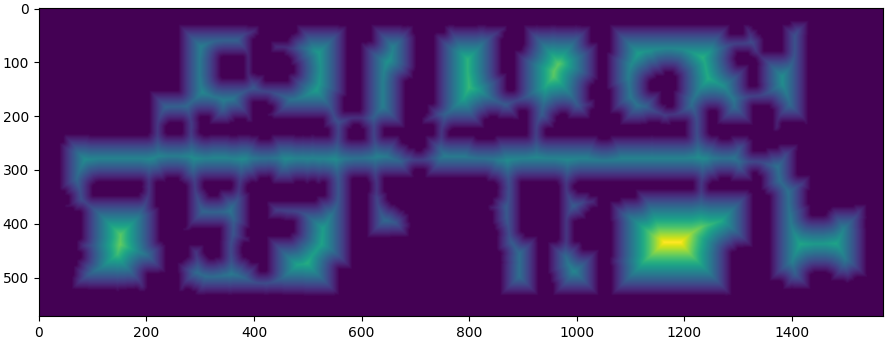
\includegraphics[width=\textwidth]{figures/50_implementation/ryu_distance_transform.png}
      \caption{Distance transform}
    \end{subfigure}%
    \begin{subfigure}{.5\textwidth}
      \centering
      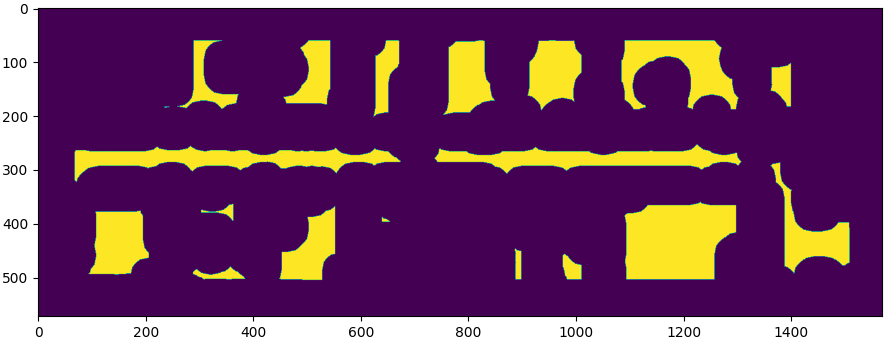
\includegraphics[width=\textwidth]{figures/50_implementation/ryu_markers.png}
      \caption{Markers as binary threshold of (a)}
    \end{subfigure}
    \caption[Distance transform and resulting markers]{Distance transform (a) and resulting markers (b) as initial information for the watershed algorithm.}
    \label{fig:distance_transform}
\end{figure}

To get the count, outlines and areas of each segment, the OpenCV function for detecting connected components is performed and returns a list of each area. With this list as input the watershed is then marker-controlled and provides a good segmentation of the whole floor into separate rooms as seen in Figure \ref{fig:watershed}.

\begin{figure}[h]
    \centering
    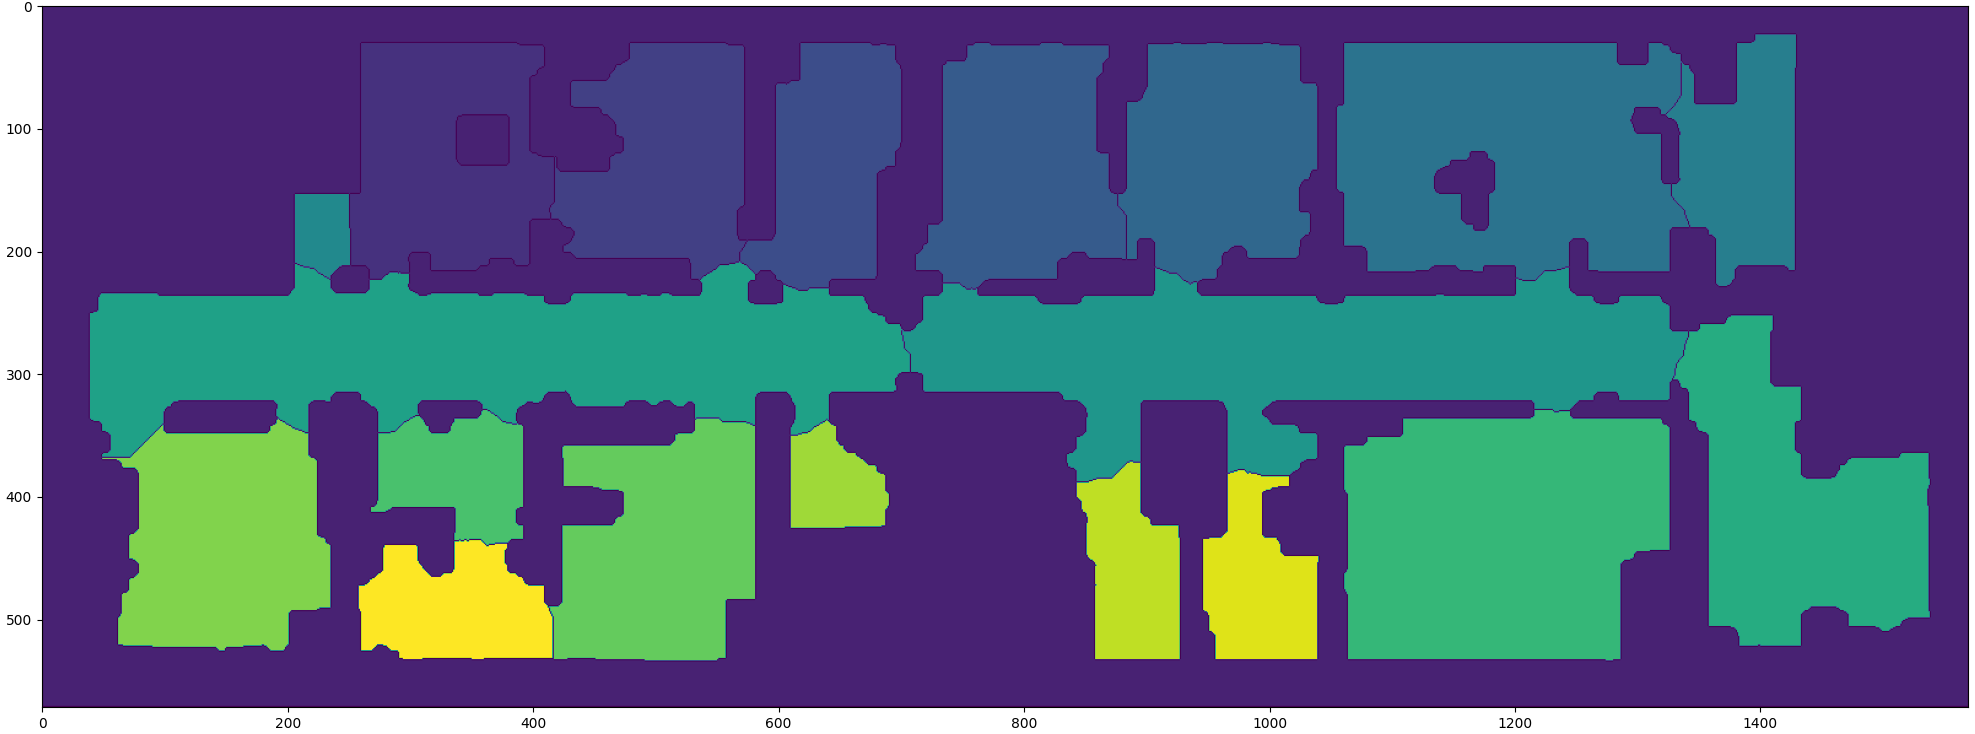
\includegraphics[width=0.75\textwidth]{figures/50_implementation/ryu_watershed.png}
    \caption[Marker-controlled watershed of the benchmark map]{Marker-controlled watershed of the benchmark map}
    \label{fig:watershed}
\end{figure}

This room segmentation provides the area for each room. To create a hierarchical graph from this the doors between them are important to create a hierarchical connection in the floor graph. The algorithm used in this work is based on the junction nodes extraction algorithm proposed by Ryu \cite{ryu_hierarchical_2020}. 

\todo{pseudocode for bridge extraction}

The base for this algorithm is the result of the watershed segmentation of Figure \ref{fig:watershed}. First, an adjacency matrix of the rooms are created. If rooms directly connect to each other with only a border created from the watershed in-between them, they have a real world connection. This connection and all pixels that lay on this border are stored. The distance transform from Figure \ref{fig:distance_transform} (a) is then taken to lookup the pixel with the maximum distance to the walls from that list of pixels on the border. Repeating this step for all connections in the adjacency matrix results in the bridge points with the maximum distance to the wall. 

\begin{figure}[h]
    \captionsetup[subfigure]{justification=centering}
    \centering
    \begin{subfigure}{.65\textwidth}
      \centering
      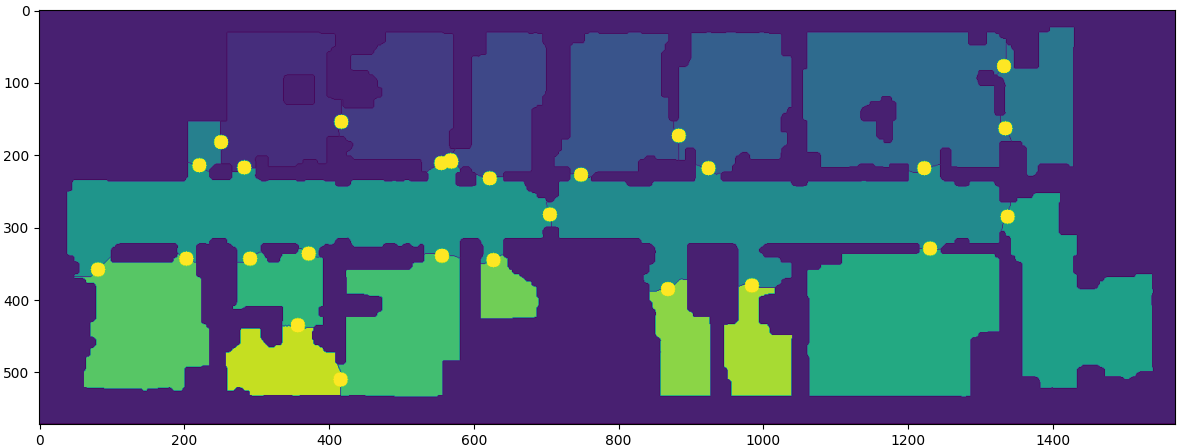
\includegraphics[width=\textwidth]{figures/50_implementation/ryu_bridge_nodes.png}
      \caption{Watershed result with detected bridge points}
    \end{subfigure}%
    \begin{subfigure}{.25\textwidth}
      \centering
      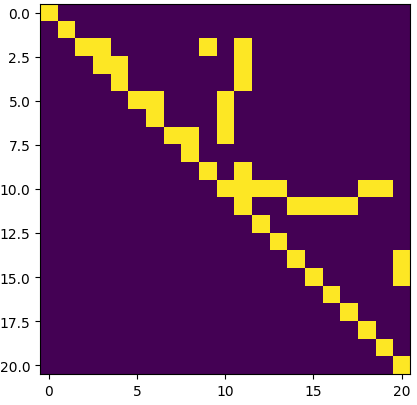
\includegraphics[width=\textwidth]{figures/50_implementation/ryu_adjacency_matrix.png}
      \caption{Adjacency matrix}
    \end{subfigure}
    \caption[The result of the bridge point detection algorithm]{The result of the bridge point detection algorithm. Bridge points overlayed on the segmented map (a). The adjacency matrix of the rooms (b). Rooms have always pixels connecting them to itself (diagonal line).}
    \label{fig:bridge_nodes}
\end{figure}

The segmented floor into rooms and their connections represented as bridge points can now be represented as a graph. Each room becomes a node in the floor graph. Each bridge point represents a door and becomes an edge in the graph. The corresponding graph can be seen in Figure \ref{fig:ryu_graph}. Note that this is inverted in the y-axis as all of the map previous images were taken from OpenCV which per default has its origin for images in the top left corner. In comparison, the graph representation is done with NetworkX which has its origin in the bottom left corner. 

\begin{figure}[h]
    \centering
    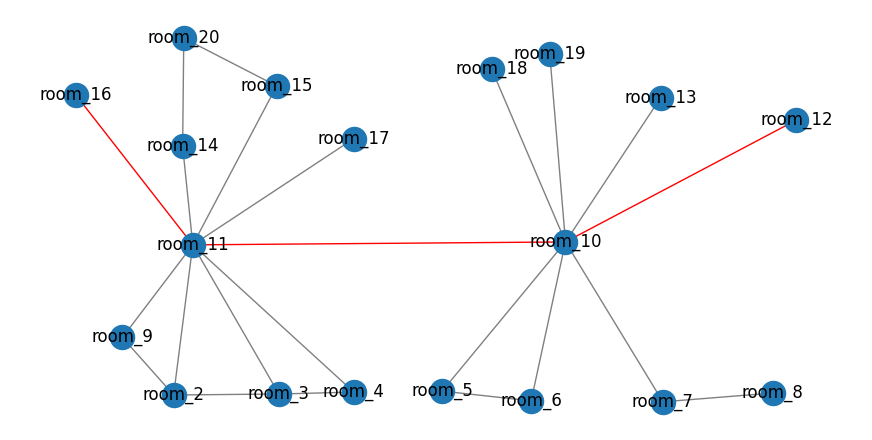
\includegraphics[width=0.7\textwidth]{figures/50_implementation/ryu_floor_graph.png}
    \caption[Graph representation of the benchmark map]{Graph representation of the benchmark map. Nodes are rooms and edges represent doors between them. In red is an example path from room 16 to room 12.}
    \label{fig:ryu_graph}
\end{figure}

To create an H-Graph for this benchmark, each room node has to hold a graph itself. These subgraphs are then the lowest hierarchical level and represent the roadmap of each room. Each Roadmap consits of collision free paths on the correspondign room-gridmap. To create this roadmap the straight path planner ILIR is used.


%% ==============================
\section{Roadmap Generation}
\label{sec:roadmap_generation}
%% ==============================
The first step for path planning is converting the environment in a Shapely object. This has the advantage, that basic shapes like lines, rectangles and polygons available, collision checks between these shapes are already implemented efficiently with a C library and the precision is higher than on the pixel based images. The images from OpenCV represent the environment in discrete pixels, this is helpful as the gridmap recorded from the laser scanners has exactly this resolution. However for collision checks and creating paths as lines it is important to precisely model these shapes. Lines should be one dimensional shapes which have no are. In comparison a line in an numpy matrix as used by OpenCV is represented in a row of pixels each with a certain width and height. This produces unexpected behavior and wrong results. The converted shapely environment can be seen in Figure \ref{fig:ryu_shapely}

\begin{figure}[h]
    \centering
    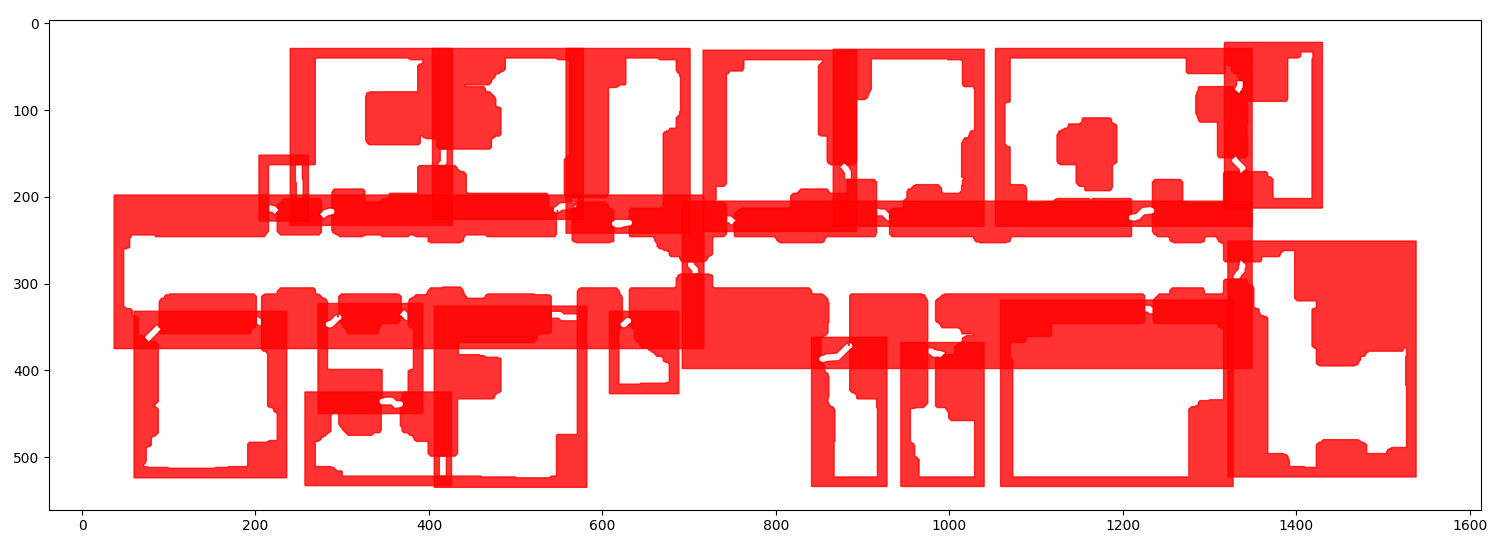
\includegraphics[width=0.75\textwidth]{figures/50_implementation/ruy_shapely.png}
    \caption[Shapely representation of the benchmark map]{Shapely representation of the benchmark map. Each room has its own environment and is surrounded by red obstacles. All room environments are drawn in one single image for visualization resulting in overlapped red obstacles.}
    \label{fig:ryu_shapely}
\end{figure}

In each room the largest interior rectangles are searched in an iterative process and combined to a polygon. The algorithm is from Marzeh et. al \cite{marzeh_algorithm_2019} and the used python implementation from Weber \cite{weber_largest_2023}. The proposed Iterative Largest Interior Rectangle (ILIR) algorithm extends these ideas by repeatedly searching the largest rectangle. Each rectangle is then substracted from the original area and the same process is done inside the remaining area. This produces not only the largest rectangle but also a polygon which is aligned to the axis of the coordinate frame. Just finding the largest interior polygon would not be useful as with high resolution this would just approximate the original shape. Also the edges of this polygon would not be parallel to the walls of the room which is an important requirement for the proposed algorithm. In Algorithm \ref{} the pseudo code of the ILIR path planner is shown.

LISTING Roadmap generation pseudocode of ILIR

FIGURE Result of ILIR in shapely environment with path 

Collision chekc in shapely environment

Mention Completness and Optimality

%% ==============================
\section{Hierarchical Planning}
\label{sec:impl_hierarchical_planning}
%% ==============================


Pseudocode of recursive planning function

Time complexity of Dijstra and recursion

Mention Completness and Optimality


% https://stackoverflow.com/questions/13467674/determining-complexity-for-recursive-functions-big-o-notation

% Bounds of the running time of Dijkstra's algorithm on a graph with edges {{mvar|E}} and vertices {{mvar|V}} can be expressed as a function of the number of edges, denoted <math>|E|</math>, and the number of vertices, denoted <math>|V|</math>, using [[big-O notation]]. 
% The simplest version of Dijkstra's algorithm stores the vertex set {{mvar|Q}} as a linked list or array, and edges as an [[adjacency list]] or [[Adjacency matrix|matrix]]. In this case, extract-minimum is simply a linear search through all vertices in {{mvar|Q}}, so the running time is <math>\Theta(|E| + |V|^2) = \Theta(|V|^2)</math>.

% For [[sparse graph]]s, that is, graphs with far fewer than <math>|V|^2</math> edges, Dijkstra's algorithm can be implemented more efficiently by storing the graph in the form of adjacency lists and using a [[self-balancing binary search tree]], [[binary heap]], [[pairing heap]], or [[Fibonacci heap]] as a [[priority queue]] to implement extracting minimum efficiently. To perform decrease-key steps in a binary heap efficiently, it is necessary to use an auxiliary data structure that maps each vertex to its position in the heap, and to keep this structure up to date as the priority queue {{mvar|Q}} changes. With a self-balancing binary search tree or binary heap, the algorithm requires
% :<math>\Theta((|E| + |V|) \log |V|)</math>
% time in the worst case (where <math>\log</math> denotes the binary logarithm <math>\log_2</math>); for connected graphs this time bound can be simplified to <math>\Theta( | E | \log | V | )</math>.  The [[Fibonacci heap]] improves this to
% :<math>\Theta(|E| + |V| \log|V|).</math>

%% ==============================
\section{Multi-Floor Navigation with Behavior Trees}
\label{sec:multi_floor_behavior_trees}
%% ==============================

BaseMovement ROS2 Action interface for move base.

Trick to set mapframe to target floor to give information fpr hierarchical planning.

Pseudocode or interface of the cpp plugin

Behavior tree for multi floor navigation


